\documentclass[11pt,reqno]{amsart}

\usepackage[margin=1.1in]{geometry}
\usepackage{amsmath,amssymb,amsthm,mathtools}
\usepackage{microtype}
\usepackage{tikz}
\usetikzlibrary{arrows.meta,positioning,calc}
\usepackage[hidelinks]{hyperref}

\theoremstyle{plain}
\newtheorem{theorem}{Theorem}[section]
\newtheorem{proposition}[theorem]{Proposition}
\newtheorem{lemma}[theorem]{Lemma}
\newtheorem{corollary}[theorem]{Corollary}
\newtheorem{question}[theorem]{Question}
\theoremstyle{definition}
\newtheorem{definition}[theorem]{Definition}
\newtheorem{example}[theorem]{Example}
\theoremstyle{remark}
\newtheorem{remark}[theorem]{Remark}

\newtheorem{theoremA}{Theorem A}
\newtheorem{theoremB}{Theorem B}
\newtheorem{theoremC}{Theorem C}
\newtheorem{theoremD}{Theorem D}
\renewcommand{\thetheoremA}{}
\renewcommand{\thetheoremB}{}
\renewcommand{\thetheoremC}{}
\renewcommand{\thetheoremD}{}

\newcommand{\restr}{\mathbin{\upharpoonright}}
\newcommand{\wdt}{\operatorname{width}}
\newcommand{\hgt}{\operatorname{height}}
\newcommand{\cl}{\omega}
\newcommand{\T}{\mathbb T}
\newcommand{\R}{\mathbb R}
\newcommand{\Z}{\mathbb Z}

\begin{document}
	
	\title[Simultaneous Borel saturation]{Simultaneous Borel saturation for chains
		and antichains, and the prescription problem}
	
	\author{}
	\address{}
	\email{}
	
	\subjclass[2020]{03E15, 06A07, 05C15, 05C69}
	
	\keywords{Dilworth's theorem, Mirsky's theorem, Greene--Kleitman theorem,
		saturated partition, Borel graph, Borel chromatic number}
	
	\begin{abstract}
		We prove that every Borel partial order admits, for each $r\ge1$, a Borel
		partition into chains which is simultaneously $r$- and $(r+1)$-saturated in
		the sense of Greene and Kleitman, and, if its height is finite, a Borel
		partition into antichains which is simultaneously saturated for the dual
		norms. Both statements, and both proofs, are instances of a single theorem
		about Borel graphs whose only inputs are the Greene--Kleitman theorem for
		finite induced subgraphs and the existence of exact Borel colourings. We then
		study the prescription problem: given finitely many disjoint Borel blocks,
		when do they extend to a Borel partition into independent sets? For two blocks
		the finite obstruction is the only one, by a parity argument which again
		covers chains and antichains simultaneously. For more than two blocks we
		isolate two hypotheses under which the same conclusion holds, and we show that
		they cannot be weakened to the finite obstruction alone: there is a Borel
		partial order of height three with three prescribed antichains satisfying both
		the finite extension property and the saturation hypothesis, but admitting no
		Borel extension. The corresponding question for chains is left open.
	\end{abstract}
	
	\maketitle
	
	\section{Introduction}
	\label{sec:intro}
	
	Dilworth's theorem is one of the basic duality principles in the theory of
	partially ordered sets. In its classical finite form, it says that the width of
	a poset, namely the maximum size of an antichain, is equal to the least number
	of chains needed to partition the poset~\cite{Dilworth1950}. Equivalently, a
	finite poset of width $n$ admits a partition into $n$ chains. This result has
	served as a point of contact between order theory, matching theory, extremal set
	theory, and, more recently, descriptive combinatorics.
	
	There are two natural directions in which Dilworth's theorem has been extended.
	The first is definability-theoretic. If the underlying set is a standard Borel
	space and the order relation is Borel, one may ask whether a purely
	combinatorial chain decomposition can be chosen in a Borel way. Harrington,
	Marker, and Shelah proved a fundamental countable-width theorem: a thin Borel
	partial order is a union of countably many Borel
	chains~\cite{HarringtonMarkerShelah1988}. In particular, a Borel partial order
	with no uncountable antichain, and hence every Borel partial order of countable
	width, admits a countable Borel chain cover. Their theorem fits naturally into
	the general pattern of descriptive-set-theoretic dichotomies: either a definable
	object admits a definable countable decomposition, or it contains a large
	perfect obstruction. This point of view was later clarified through the
	graph-theoretic approach to descriptive set theory. Applied to the
	incomparability graph of a partial order, the Kechris--Solecki--Todorcevic $G_0$
	dichotomy gives a topological route to countable Borel decompositions and
	perfect antichain alternatives~\cite{KechrisSoleckiTodorcevic1999}. Miller's
	work emphasized that many classical dichotomy theorems, including the
	Harrington--Marker--Shelah phenomenon, can be reproved and generalized by
	isolating the appropriate Borel graph and then using Baire category
	arguments~\cite{Miller2012}. At the finite-width level, Kada obtained a Borel
	version of Dilworth's theorem, and Carroy, Miller, and Vidny\'anszky later gave
	a broad definable strengthening: under suitable definability hypotheses, either a
	quasi-order is covered by $k$ Borel chains or it contains an antichain of size
	$k+1$~\cite{Kada1989, CarroyMillerVidnyanszky2021}.
	
	The second direction is finite-combinatorial. Greene and Kleitman refined
	Dilworth's theorem by replacing antichains with unions of several disjoint
	antichains~\cite{GreeneKleitman1976}. If $P$ is a finite poset and $t\ge1$, let
	\[
	\alpha_t(P)
	=\max\bigl\{|A_0\cup\cdots\cup A_{t-1}|:
	A_0,\ldots,A_{t-1}\ \text{are pairwise disjoint antichains}\bigr\}.
	\]
	For a chain partition $\mathcal C$ of $P$, define
	\[
	\lVert\mathcal C\rVert_t=\sum_{C\in\mathcal C}\min\{|C|,t\}.
	\]
	This quantity is an upper bound for $\alpha_t(P)$. A chain partition is called
	$t$-saturated if equality holds. Dilworth's theorem is precisely the case
	$t=1$. Greene and Kleitman proved the stronger simultaneous statement that, for
	every $t$, every finite poset has a chain partition which is both $t$-saturated
	and $(t+1)$-saturated. Simultaneity is the whole point: it is what makes the
	result a theorem rather than a sequence of independent optimisations, and all
	known proofs of it are finitary~\cite{GreeneKleitman1976, Greene1976, Saks1979,
		Frank1980}. Mirsky's theorem~\cite{Mirsky1971}, that a poset of height $h$ is a
	union of $h$ antichains, is the case $t=1$ of the dual refinement, obtained by
	interchanging the roles of chains and antichains throughout.
	
	The purpose of this paper is to bring these two directions together. We ask
	whether the Greene--Kleitman saturation phenomenon persists for infinite posets,
	and whether, in the definable setting, the saturated chain partition can be
	chosen Borel. Thus the question is not merely whether a finite-width Borel poset
	can be decomposed into the optimal number of Borel chains, but whether such a
	decomposition can also realize the Greene--Kleitman norms simultaneously. Our
	first result is the corresponding refinement.
	
	\begin{theoremA}
		Let $P$ be a Borel partial order on a standard Borel space $X$, and let
		$r\ge1$. Then $X$ admits a Borel partition into chains which is
		simultaneously $r$- and $(r+1)$-saturated. If moreover $P$ has finite height,
		then $X$ admits a Borel partition into antichains which is simultaneously
		$r$- and $(r+1)$-saturated for the dual norms.
	\end{theoremA}
	
	The two halves of Theorem A are proved at once. That Dilworth's and Mirsky's
	theorems are two readings of a single graph-theoretic phenomenon is classical:
	Mirsky's theorem says that a comparability graph satisfies $\chi=\cl$, and
	Dilworth's that the complement of a comparability graph does, and both are
	subsumed by the perfectness of comparability
	graphs~\cite{Berge1961,Lovasz1972}. On the Greene--Kleitman side, the passage
	from orders to graphs and digraphs was begun by Linial~\cite{Linial1981} and
	Berge~\cite{Berge1982} and pursued by Cameron~\cite{Cameron1986} and
	Frank~\cite{Frank1980}; we make no use of their results, but we take from them
	the formulation. Throughout, then, chains and antichains are read as independent
	sets and cliques of the incomparability graph, or of the comparability graph as
	the case requires, and Theorem A becomes a statement about Borel graphs
	(Theorem~\ref{thm:main-saturation}) resting on exactly two hypotheses: the
	Greene--Kleitman theorem for the finite induced subgraphs of $G$, and the
	existence of exact Borel colourings of the Borel induced subgraphs of $G$. The
	first is finite combinatorics, the second is the Borel Dilworth or Borel Mirsky
	theorem. The proof, in \S\ref{sec:saturation}, extracts from the finite theorem a
	finite \emph{locked template} whose \emph{active blocks} carry all of the norms,
	and then replaces the active blocks by an exact Borel colouring of the set they
	span.
	
	That last step replaces the active blocks; it does not preserve them. This is
	what leads to the second half of the paper, \S\ref{sec:prescription}. Call a
	family $E_0,\dots,E_{k-1}$ of pairwise disjoint independent Borel sets a
	\emph{prescription}, and ask whether it extends to a Borel partition
	$X=A_0\sqcup\dots\sqcup A_{k-1}$ into independent sets with $E_i\subseteq A_i$.
	There is an evident finite obstruction, and by compactness it is the only
	obstruction to the existence of an extension in the abstract, without
	definability: the prescription extends abstractly if and only if it extends on
	every finite set, a property we call $\mathrm{(FE)}_k$
	(Proposition~\ref{prop:compactness}). The question is whether $\mathrm{(FE)}_k$
	also suffices in the Borel category.
	
	For $k=2$ it does, and again for chains and antichains at once.
	
	\begin{theoremB}
		Let $G$ be a Borel graph on a standard Borel space $X$ admitting a Borel
		proper $2$-colouring, and let $E_0,E_1$ be a prescription satisfying
		$\mathrm{(FE)}_2$. Then $E_0,E_1$ extends to a Borel partition of $X$ into two
		independent sets. In particular this holds for the chains of a Borel order of
		width two and for the antichains of a Borel order of height two.
	\end{theoremB}
	
	The proof, in \S\ref{subsec:two}, is a cocycle argument: any Borel proper
	$2$-colouring differs from the desired one by a flip which is constant on each
	connected component, $\mathrm{(FE)}_2$ says that the prescribed flip is well
	defined, and Burgess's invariant separation theorem~\cite{Burgess1979} makes it
	Borel. Only the weakest form of $\mathrm{(FE)}_2$ is used, namely its
	restriction to the vertex sets of paths, which we show to be equivalent to a
	bare parity condition. The hypothesis that $G$ be Borel $2$-colourable cannot be
	dropped, as the Schreier graph of an irrational rotation shows
	(Remark~\ref{rem:rotation}); in the two applications it is supplied for free.
	
	For $k\ge3$ the cocycle has no substitute, and we proceed by iterated
	puncturing. Two hypotheses on the prescription appear: \emph{anchor saturation}
	$\mathrm{(AS)}$, that every prescribed point lie on a $k$-clique meeting each
	$E_i$ once, and \emph{anchored decomposition} $\mathrm{(AD)}$, a form of
	$\mathrm{(FE)}$ for the tail index sets $\{t,\dots,k-1\}$.
	
	\begin{theoremC}
		Let $G$ be a Borel graph, $k\ge1$, and let $E_0,\dots,E_{k-1}$ be a
		prescription by finite sets satisfying $\mathrm{(AS)}$ and $\mathrm{(AD)}$.
	Then the
		prescription extends to a Borel partition into $k$ independent sets.
	\end{theoremC}
	
	Hypothesis $\mathrm{(AD)}$ is genuinely stronger than $\mathrm{(FE)}_k$, and not
	by an artefact of the proof. Our last result exhibits the gap, and it does so on
	the antichain side, where a counterexample can be built.
	
	\begin{theoremD}
		There are a Borel partial order of height three on a standard Borel space and
		a prescription $E_0,E_1,E_2$ by three-element antichains which satisfies
		$\mathrm{(FE)}_3$ and $\mathrm{(AS)}$, but which extends to no Borel partition
		into three antichains. 
	\end{theoremD}
	
	The construction, in \S\ref{subsec:counterexample}, encodes the irrational
	rotation graph into a height-three order by a gadget which forces every anchored
	proper $3$-colouring to induce a proper $2$-colouring of the rotation graph; the
	saturation hypothesis is then arranged by attaching a three-element chain above
	each prescribed point. That this attachment is possible at all is the real
	content of Theorem D: for antichains, $\mathrm{(AS)}$ is a hypothesis one can
	always install, and hence carries no information by itself. For chains it
	cannot be installed, because one would have to attach incomparabilities, which
	propagate, and width is a global constraint. We do not know whether
	$\mathrm{(FE)}_3$ and $\mathrm{(AS)}$ suffice for three chains, and
	\S\ref{subsec:open} explains what a counterexample would have to look like.
	
	\subsection*{Notation}
	
	All spaces are standard Borel. A \emph{graph} on $X$ is a symmetric irreflexive
	relation $G\subseteq X^2$; we write $x\,G\,y$ for $(x,y)\in G$ and
	$G\restr Y=G\cap(Y\times Y)$. For a partial order $P=(X,\le_P)$ we write
	$x\perp_Py$ for ``$x\neq y$ and $x,y$ are $\le_P$-incomparable''. We put
	$[k]=\{0,\dots,k-1\}$, and for $a,b\in\{0,1\}$ we let $a\oplus b$ be addition
	modulo $2$ and $\mathbf1_H$ the characteristic function of $H$. Partitions
	indexed by a set are allowed to have empty parts; unindexed partitions have
	none.
	
	\section{Cliques, independent sets, and saturation}
	\label{sec:prelim}
	
	Let $G$ be a graph on $X$. A set $I\subseteq X$ is \emph{independent} if no two
	of its points are $G$-adjacent, and $K\subseteq X$ is a \emph{clique} if any two
	distinct points of $K$ are. We write
	\[
	\cl(Y)=\sup\{|K|:K\subseteq Y\ \text{a clique}\}
	\]
	for the clique number of $G\restr Y$, and for $t\ge1$
	\[
	\cl_t(Y)=\sup\bigl\{|K_0\cup\dots\cup K_{t-1}|:
	K_0,\dots,K_{t-1}\subseteq Y\ \text{pairwise disjoint cliques}\bigr\}.
	\]
	Thus $\cl_1=\cl$, and $\cl_t(Y)\le t\,\cl(Y)$, so that all the $\cl_t(Y)$ are
	finite as soon as $\cl(Y)$ is, in which case the suprema are attained. An
	\emph{independent partition} of $Y$ is a partition of $Y$ all of whose blocks
	are independent, and its \emph{$t$-norm} is
	\[
	\lVert\mathcal P\rVert_t=\sum_{I\in\mathcal P}(|I|\wedge t),
	\qquad |I|\wedge t=\min(|I|,t),
	\]
	with $|I|\wedge t=t$ for infinite $I$. We call $\mathcal P$ \emph{$t$-saturated}
	if $\lVert\mathcal P\rVert_t=\cl_t(Y)$, and \emph{simultaneously
		$(r,r{+}1)$-saturated} if it is $r$- and $(r{+}1)$-saturated.
	
	\begin{lemma}[Weak duality]
		\label{lem:weak-duality}
		For every $Y\subseteq X$, every independent partition $\mathcal P$ of $Y$ and
		every $t\ge1$ one has $\cl_t(Y)\le\lVert\mathcal P\rVert_t$.
	\end{lemma}
	
	\begin{proof}
		Let $K_0,\dots,K_{t-1}\subseteq Y$ be pairwise disjoint cliques and
		$T=K_0\cup\dots\cup K_{t-1}$. An independent set meets a clique in at most one
		point, so $|I\cap T|\le t$ for every $I\in\mathcal P$; as also
		$|I\cap T|\le|I|$, we get $|I\cap T|\le|I|\wedge t$ and hence
		$|T|=\sum_{I}|I\cap T|\le\lVert\mathcal P\rVert_t$. Take the supremum over
		packings.
	\end{proof}
	
	Fix now an algebra $\mathcal A$ of subsets of $X$ containing the singletons; in
	all applications $\mathcal A$ is either the $\sigma$-algebra of Borel sets or the
	power set of $X$. Two hypotheses on $(G,\mathcal A)$ will be used.
	
	\begin{itemize}
		\item[$\mathrm{(FS)}$] \emph{Finite saturation.} For every finite
		$F\subseteq X$ and every $r\ge1$ the graph $G\restr F$ has a simultaneously
		$(r,r{+}1)$-saturated independent partition.
		\item[$\mathrm{(EC)}$] \emph{Exact colouring.} For every $Y\in\mathcal A$ the
		graph $G\restr Y$ has an independent partition into $\cl(Y)$ blocks, all
		belonging to $\mathcal A$.
	\end{itemize}
	
	\subsection*{Examples}
	
	Let $P=(X,\le_P)$ be a partial order, and let
	\[
	G^{\perp}=\{(x,y):x\perp_Py\},
	\qquad
	G^{<}=\{(x,y):x<_Py\ \text{or}\ y<_Px\}
	\]
	be its incomparability and comparability graphs. Independent sets of
	$G^{\perp}$ are the chains of $P$ and its cliques the antichains, so
	$\cl(G^{\perp})=\wdt(P)$, $\cl_t=\alpha_t$, independent partitions are chain
	partitions and $\lVert\cdot\rVert_t$ is the Greene--Kleitman norm. Dually,
	independent sets of $G^{<}$ are the antichains and its cliques the chains,
	$\cl(G^{<})=\hgt(P)$, $\cl_t=\beta_t$, and $\lVert\cdot\rVert_t$ is the dual
	norm. Under this dictionary, $\mathrm{(FS)}$ for $G^{\perp}$ is the
	Greene--Kleitman theorem~\cite{GreeneKleitman1976} applied to the finite induced
	subposets, and for $G^{<}$ its antichain dual; $\mathrm{(EC)}$ with
	$\mathcal A=\mathcal P(X)$ is Dilworth's, resp.\ Mirsky's, theorem for orders of
	finite width, resp.\ height, and with $\mathcal A$ Borel it is the Borel
	Dilworth, resp.\ Borel Mirsky, theorem~\cite{Kada1989,
		CarroyMillerVidnyanszky2021}. In the Borel cases $\mathrm{(EC)}$ holds for
	\emph{every} Borel $Y$, since $P\restr Y$ is again a Borel partial order on a
	standard Borel space of no larger width, resp.\ height.
	
	\section{Simultaneous saturation}
	\label{sec:saturation}
	
	Throughout this section $G$ is a graph on $X$ with $\cl(X)<\infty$ satisfying
	$\mathrm{(FS)}$, and $r\ge1$ is fixed. Write $a_r=\cl_r(X)$ and
	$a_{r+1}=\cl_{r+1}(X)$, both finite, and fix pairwise disjoint cliques
	$K_0,\dots,K_{r-1}$ and $L_0,\dots,L_r$ with
	\[
	U=K_0\cup\dots\cup K_{r-1},\quad |U|=a_r,
	\qquad
	V=L_0\cup\dots\cup L_r,\quad |V|=a_{r+1},
	\]
	and set $S=U\cup V$, a finite set. Since the two packings lie in every
	$Z\supseteq S$ while every $Z\subseteq X$ obeys the global bounds,
	\begin{equation}
		\cl_r(Z)=a_r
		\qquad\text{and}\qquad
		\cl_{r+1}(Z)=a_{r+1}
		\qquad (S\subseteq Z\subseteq X).
		\label{eq:norms-stable}
	\end{equation}
	For a partition $\mathcal D$ of $Z\supseteq S$ put
	$\mathcal D\restr S=\{D\cap S:D\in\mathcal D,\ D\cap S\neq\varnothing\}$; we say
	$\mathcal D$ \emph{extends} $\mathcal E$ if $\mathcal D\restr S=\mathcal E$.
	
	The following is the device that transfers finite information to the whole
	space. Its proof is a finite intersection argument, made possible by the
	finiteness of $S$.
	
	\begin{lemma}[Locked template]
		\label{lem:locked}
		There is an independent partition $\mathcal E$ of $S$ such that for every
		finite $F\subseteq X\setminus S$ some independent partition of $S\cup F$
		extends $\mathcal E$ and has $r$-norm $a_r$ and $(r{+}1)$-norm $a_{r+1}$.
	\end{lemma}
	
	\begin{proof}
		Let $\Pi$ be the set of independent partitions of $S$, a finite set, and for
		finite $F\subseteq X\setminus S$ let $\Pi_F$ consist of those
		$\mathcal E\in\Pi$ admitting such an extension over $S\cup F$.
		
		Each $\Pi_F$ is nonempty. By $\mathrm{(FS)}$ the finite graph
		$G\restr(S\cup F)$ has a simultaneously $(r,r{+}1)$-saturated independent
		partition $\mathcal D$, whose norms are $a_r$ and $a_{r+1}$ by
		\eqref{eq:norms-stable}; then $\mathcal D\restr S\in\Pi_F$.
		
		The family is monotone: $F\subseteq F'$ implies $\Pi_{F'}\subseteq\Pi_F$.
		Indeed, if $\mathcal D'$ witnesses $\mathcal E\in\Pi_{F'}$, then the
		restriction $\mathcal D$ of $\mathcal D'$ to $S\cup F$ is an independent
		partition extending $\mathcal E$, and from
		$|D'\cap(S\cup F)|\wedge t\le|D'|\wedge t$ we get
		$\lVert\mathcal D\rVert_t\le\lVert\mathcal D'\rVert_t$ for $t\in\{r,r+1\}$,
		while Lemma~\ref{lem:weak-duality} and \eqref{eq:norms-stable} give the reverse
		inequalities; so both norms are again $a_r$ and $a_{r+1}$.
		
		Finally $\bigcap_F\Pi_F\neq\varnothing$. Otherwise choose for each
		$\mathcal E\in\Pi$ a finite $F_{\mathcal E}\subseteq X\setminus S$ with
		$\mathcal E\notin\Pi_{F_{\mathcal E}}$; then
		$F^{*}=\bigcup_{\mathcal E\in\Pi}F_{\mathcal E}$ is finite, and any
		$\mathcal E^{*}\in\Pi_{F^{*}}$ satisfies
		$\mathcal E^{*}\in\Pi_{F_{\mathcal E^{*}}}$ by monotonicity, a contradiction.
		Any member of the intersection is as required.
	\end{proof}
	
	Fix such an $\mathcal E$ for the remainder of the section. Taking
	$F=\varnothing$ gives
	\begin{equation}
		\lVert\mathcal E\rVert_r=a_r,
		\qquad
		\lVert\mathcal E\rVert_{r+1}=a_{r+1}.
		\label{eq:template-norms}
	\end{equation}
	
	\begin{definition}
		\label{def:active}
		A block $E\in\mathcal E$ is \emph{active} if $|E\cap U|=r$ and
		$|E\cap V|=r+1$. We list the active blocks as $E_0,\dots,E_{\ell-1}$ and put
		$E_I=\bigcup_{i\in I}E_i$ for $I\subseteq[\ell]$.
	\end{definition}
	
	\begin{lemma}
		\label{lem:active-points}
		For all $i<\ell$, $j<r$ and $j'\le r$ the sets $E_i\cap K_j$ and
		$E_i\cap L_{j'}$ are singletons, say $\{e_i^{\,j}\}$ and $\{f_i^{\,j'}\}$.
		Consequently $|E_i|\wedge r=r$ and $|E_i|\wedge(r+1)=r+1$, and for each $j<r$
		and $j'\le r$ the sets
		\[
		\widetilde K_j=\{e_p^{\,j}:p<\ell\},
		\qquad
		\widetilde L_{j'}=\{f_p^{\,j'}:p<\ell\}
		\]
		are cliques of cardinality $\ell$ meeting every active block in exactly one
		point.
	\end{lemma}
	
	\begin{proof}
		$E_i$ is independent and $K_j$ is a clique, so $|E_i\cap K_j|\le1$; since
		$U=\bigsqcup_{j<r}K_j$ and $|E_i\cap U|=r$, all $r$ intersections are
		singletons, and likewise for $V=\bigsqcup_{j'\le r}L_{j'}$. The sets
		$\widetilde K_j$ have $\ell$ elements because the active blocks are pairwise
		disjoint, and are cliques as subsets of $K_j$.
	\end{proof}
	
	\begin{lemma}
		\label{lem:active-decomposition}
		For every finite $F\subseteq X\setminus S$ there is a partition
		$F=F_0\sqcup\dots\sqcup F_{\ell-1}$ with $E_i\cup F_i$ independent for each
		$i<\ell$. In particular $\ell=0$ forces $X=S$.
	\end{lemma}
	
	\begin{proof}
		Let $\mathcal D$ extend $\mathcal E$ over $S\cup F$ with norms $a_r$ and
		$a_{r+1}$. Every $D\in\mathcal D$ is independent and $U$ is a union of $r$
		disjoint cliques, so $|D\cap U|\le|D|\wedge r$ as in
		Lemma~\ref{lem:weak-duality}; summing over $\mathcal D$,
		\[
		a_r=|U|=\sum_{D\in\mathcal D}|D\cap U|
		\le\sum_{D\in\mathcal D}(|D|\wedge r)=\lVert\mathcal D\rVert_r=a_r,
		\]
		whence $|D\cap U|=|D|\wedge r$ for every $D$, and likewise
		$|D\cap V|=|D|\wedge(r+1)$.
		
		Let $D\in\mathcal D$ meet $F$. If $|D\cap U|<r$ then $|D|\wedge r<r$, so
		$|D|\wedge r=|D|$ and $D=D\cap U\subseteq S$, contradicting
		$D\cap F\neq\varnothing$; hence $|D\cap U|=r$, and $|D\cap V|=r+1$ for the same
		reason. As $U,V\subseteq S$ and $\mathcal D$ extends $\mathcal E$, the trace
		$D\cap S$ is an active block.
		
		For $i<\ell$ let $D_i$ be the unique block of $\mathcal D$ with
		$D_i\cap S=E_i$, and set $F_i=D_i\cap F$. By the previous paragraph the $D_i$
		cover $F$, so $F=F_0\sqcup\dots\sqcup F_{\ell-1}$, and
		$E_i\cup F_i\subseteq D_i$ is independent. If $\ell=0$ then every finite
		$F\subseteq X\setminus S$ is empty, i.e.\ $X=S$.
	\end{proof}
	
	From now on put $Y=(X\setminus S)\cup E_{[\ell]}$, so that
	$Y\cap S=E_{[\ell]}$.
	
	\begin{lemma}
		\label{lem:clique-number}
		$\cl(Y)=\ell$.
	\end{lemma}
	
	\begin{proof}
		A clique of size $\ell+1$ contains a finite one, so it suffices to bound
		finite cliques. Let $K\subseteq Y$ be a finite clique and $F=K\setminus S$;
		decomposing $F=F_0\sqcup\dots\sqcup F_{\ell-1}$ as in
		Lemma~\ref{lem:active-decomposition} and using $Y\cap S=E_{[\ell]}$ we get
		$K\subseteq\bigcup_{i<\ell}(E_i\cup F_i)$, and each $E_i\cup F_i$ is
		independent, hence meets $K$ at most once; so $|K|\le\ell$. Conversely, if
		$\ell>0$ then $\widetilde K_0\subseteq E_{[\ell]}\subseteq Y$ is a clique of
		size $\ell$ by Lemma~\ref{lem:active-points}, while if $\ell=0$ then $Y$ is
		empty by Lemma~\ref{lem:active-decomposition}.
	\end{proof}
	
	\begin{theorem}
		\label{thm:main-saturation}
		Let $X$ be a set, $\mathcal A$ an algebra of subsets of $X$ containing the
		singletons, and $G$ a graph on $X$ with $\cl(X)<\infty$ satisfying
		$\mathrm{(FS)}$ and $\mathrm{(EC)}$. Then for every $r\ge1$ there is a finite
		independent partition $\mathcal C$ of $X$, with all blocks in $\mathcal A$,
		such that
		\[
		\lVert\mathcal C\rVert_r=\cl_r(X)
		\qquad\text{and}\qquad
		\lVert\mathcal C\rVert_{r+1}=\cl_{r+1}(X).
		\]
	\end{theorem}
	
	\begin{proof}
		Fix $r$ and keep the notation above. If $\ell=0$ then $X=S$ and
		$\mathcal C=\mathcal E$ will do, its blocks being finite and
		\eqref{eq:template-norms} being the conclusion.
		
		Assume $\ell>0$. Since $S$ is finite and $\mathcal A$ is an algebra containing
		the singletons, $Y\in\mathcal A$; by Lemma~\ref{lem:clique-number}
		$\cl(Y)=\ell$, so $\mathrm{(EC)}$ provides an independent partition
		$Y=C_0\sqcup\dots\sqcup C_{\ell-1}$ with all $C_i\in\mathcal A$.
		
		Fix $j<r$. By Lemma~\ref{lem:active-points} the set $\widetilde K_j\subseteq Y$
		is a clique with $\ell$ elements, and each of the $\ell$ independent sets
		$C_i$ meets it at most once, hence exactly once. As the $K_j$ $(j<r)$ are
		pairwise disjoint, this exhibits $r$ distinct points in each $C_i$, so
		$|C_i|\wedge r=r$; running the argument with $\widetilde L_{j'}$ $(j'\le r)$
		gives $|C_i|\wedge(r+1)=r+1$. By Lemma~\ref{lem:active-points} the active
		blocks satisfy the same two equalities, so $C_0,\dots,C_{\ell-1}$ contribute to
		the two norms exactly what $E_0,\dots,E_{\ell-1}$ contribute. Since
		$X=Y\sqcup(S\setminus E_{[\ell]})$ and the inactive blocks of $\mathcal E$
		partition $S\setminus E_{[\ell]}$ into finite independent sets,
		\[
		\mathcal C=\{C_i:i<\ell\}\cup\bigl(\mathcal E\setminus\{E_i:i<\ell\}\bigr)
		\]
		is a finite independent partition of $X$ with blocks in $\mathcal A$, and by
		\eqref{eq:template-norms}
		\[
		\lVert\mathcal C\rVert_r=\lVert\mathcal E\rVert_r=a_r,
		\qquad
		\lVert\mathcal C\rVert_{r+1}=\lVert\mathcal E\rVert_{r+1}=a_{r+1}.
		\qedhere
		\]
	\end{proof}
	
	\begin{corollary}
		\label{cor:borel-chain}
		Let $P$ be a Borel partial order of finite width on a standard Borel space $X$
		and let $r\ge1$. Then $X$ has a finite Borel chain partition $\mathcal C$ with
		$\lVert\mathcal C\rVert_r=\alpha_r(X)$ and
		$\lVert\mathcal C\rVert_{r+1}=\alpha_{r+1}(X)$.
	\end{corollary}
	
	\begin{proof}
		Apply Theorem~\ref{thm:main-saturation} to $G^{\perp}$ with $\mathcal A$ the
		Borel sets; $\cl(X)=\wdt(P)<\infty$, $\mathrm{(FS)}$ is the Greene--Kleitman
		theorem and $\mathrm{(EC)}$ the Borel Dilworth theorem.
	\end{proof}
	
	\begin{corollary}
		\label{cor:borel-antichain}
		Let $P$ be a Borel partial order of finite height on a standard Borel space $X$
		and let $r\ge1$. Then $X$ has a finite Borel antichain partition
		$\mathcal A$ with $\lVert\mathcal A\rVert_r=\beta_r(X)$ and
		$\lVert\mathcal A\rVert_{r+1}=\beta_{r+1}(X)$.
	\end{corollary}
	
	\begin{proof}
		As above with $G^{<}$, using the antichain dual of the Greene--Kleitman
		theorem and the Borel Mirsky theorem.
	\end{proof}
	
	It remains to remove the finiteness assumption on the width, which is a matter
	of disposing of two degenerate cases.
	
	\begin{proposition}
		\label{prop:infinite-width}
		Let $P$ be a Borel partial order of infinite width on a standard Borel space
		$X$, and let $t\ge1$. Then $X$ has a Borel chain partition $\mathcal C$ with
		$\lVert\mathcal C\rVert_t=\alpha_t(X)$; the same $\mathcal C$ works for all
		$t$ simultaneously.
	\end{proposition}
	
	\begin{proof}
		By the Harrington--Marker--Shelah dichotomy~\cite{HarringtonMarkerShelah1988},
		either $P$ contains a perfect antichain or $X$ is covered by countably many
		Borel chains.
		
		In the first case $X$ is uncountable, so $|X|=2^{\aleph_0}$, and a perfect
		antichain has cardinality $2^{\aleph_0}$, whence
		$\alpha_t(X)=2^{\aleph_0}=|X|$ for every $t$. The partition into singletons is
		Borel and has $t$-norm $|X|$.
		
		In the second case, refining a countable Borel chain cover to a partition
		gives a Borel chain partition $\mathcal C=\{C_n:n<N\}$ with $N\le\omega$ and
		all $C_n$ nonempty. If $N$ were finite, $\wdt(P)\le N$ would be finite; so
		$N=\omega$ and $\lVert\mathcal C\rVert_t=\sum_{n<\omega}(|C_n|\wedge
		t)=\aleph_0$ for every $t$. On the other hand every antichain is countable, so
		$\alpha_t(X)\le\aleph_0$, while $\wdt(P)$ being infinite there are antichains
		of every finite size, so $\alpha_t(X)\ge\alpha_1(X)=\aleph_0$. Hence
		$\alpha_t(X)=\aleph_0=\lVert\mathcal C\rVert_t$.
	\end{proof}
	
	\begin{proof}[Proof of Theorem A]
		The chain half is Corollary~\ref{cor:borel-chain} if $\wdt(P)<\infty$ and
		Proposition~\ref{prop:infinite-width} otherwise. The antichain half is
		Corollary~\ref{cor:borel-antichain}.
	\end{proof}
	
	\begin{remark}
		\label{rem:infinite-height}
		The antichain half of Theorem A likewise holds without any assumption on the
		height as soon as one has the dual dichotomy, namely that a Borel partial
		order either contains a perfect chain or is covered by countably many Borel
		antichains: the two cases are then disposed of exactly as in
		Proposition~\ref{prop:infinite-width}. We do not know whether that dichotomy
		holds, and we do not use it.
	\end{remark}
	
	\begin{remark}
		Theorem~\ref{thm:main-saturation} uses no definability of $G$ itself; all the
		definability is concentrated in $\mathrm{(EC)}$, and is applied to the single
		set $Y$. In particular Corollaries~\ref{cor:borel-chain}
		and~\ref{cor:borel-antichain} hold for co-analytic partial orders as well,
		granted $\mathrm{(EC)}$ for those, since a locked template and its active
		blocks are finite objects. Taking $\mathcal A=\mathcal P(X)$ recovers the
		Greene--Kleitman theorem for arbitrary orders of finite width, and its dual,
		in the form of Aharoni and Korman~\cite{AharoniKorman1992}.
	\end{remark}
	
	\section{The prescription problem}
	\label{sec:prescription}
	
	The proof of Theorem~\ref{thm:main-saturation} discards the active blocks: the
	sets $C_i$ produced by $\mathrm{(EC)}$ agree with $E_i$ in no way beyond
	carrying the same contribution to the two norms. It is natural to ask for more,
	and this section is devoted to the resulting question.
	
	\subsection{Prescriptions and the finite obstruction}
	\label{subsec:prescription}
	
	\begin{definition}
		\label{def:prescription}
		Let $G$ be a graph on $X$ and $k\ge1$. A \emph{prescription} is a family
		$E_0,\dots,E_{k-1}$ of pairwise disjoint independent subsets of $X$. It
		\emph{extends} to a partition $X=A_0\sqcup\dots\sqcup A_{k-1}$ into
		independent sets if $E_i\subseteq A_i$ for all $i<k$. We say the prescription
		has the \emph{finite extension property} $\mathrm{(FE)}_k$ if for every finite
		$F\subseteq X$ there is a partition $F=D_0\sqcup\dots\sqcup D_{k-1}$ into
		$G\restr F$-independent sets with $F\cap E_i\subseteq D_i$ for all $i<k$.
	\end{definition}
	
	$\mathrm{(FE)}_k$ is plainly necessary for an extension to exist. It is also
	sufficient, if no definability is demanded.
	
	\begin{proposition}
		\label{prop:compactness}
		A prescription $E_0,\dots,E_{k-1}$ extends if and only if it satisfies
		$\mathrm{(FE)}_k$.
	\end{proposition}
	
	\begin{proof}
		Necessity is immediate, on taking $D_i=F\cap A_i$. For sufficiency give
		$k^X=\{0,\dots,k-1\}^X$ the product topology, so that it is compact, and
		consider the closed sets $O_{x,y}=\{f:f(x)\neq f(y)\}$ for $x\,G\,y$ and
		$O_{e,i}=\{f:f(e)=i\}$ for $i<k$ and $e\in E_i$. Given finitely many of them,
		let $F$ be the finite set of points they mention, take
		$F=D_0\sqcup\dots\sqcup D_{k-1}$ as in $\mathrm{(FE)}_k$ and let $f$ be any
		extension of the map sending $x\in D_i$ to $i$. If $x\,G\,y$ with $x,y\in F$
		then $x,y$ lie in different $D_i$, these being independent in $G\restr F$, so
		$f(x)\neq f(y)$; and $f(e)=i$ for $e\in E_i\cap F$. Thus the family has the
		finite intersection property, and any $f$ in the total intersection yields
		$A_i=f^{-1}(\{i\})$.
	\end{proof}
	
	The question is therefore whether $\mathrm{(FE)}_k$ suffices in the Borel
	category. For $G^{\perp}$ it reads: given disjoint Borel chains $E_i$ such that
	every finite set can be split into $k$ chains respecting the prescription, is
	there a Borel partition of $X$ into $k$ chains extending it? And dually for
	antichains.
	
	\subsection{Two blocks}
	\label{subsec:two}
	
	For $k=2$ the answer is affirmative, and the argument is a single cocycle
	computation which sees neither chains nor antichains. Moreover only the weakest
	form of $\mathrm{(FE)}_2$ is needed, namely its restriction to paths, which is
	equivalent to a bare parity condition. Recall that a \emph{$G$-path of length
		$n$} from $x$ to $y$ is a tuple $(x_0,\dots,x_n)$ with $x_0=x$, $x_n=y$ and
	$x_m\,G\,x_{m+1}$ for $m<n$, and that $E_G$, the relation of being joined by a
	$G$-path, is the connectedness relation of $G$, an analytic equivalence relation
	when $G$ is Borel.
	
	\begin{theorem}
		\label{thm:two}
		Let $G$ be a Borel graph on a standard Borel space $X$ admitting a Borel
		proper $2$-colouring, and let $E_0,E_1\subseteq X$ be disjoint Borel sets. The
		following are equivalent.
		\begin{enumerate}
			\item[(i)] $E_0,E_1$ extends to a partition of $X$ into two Borel
			independent sets.
			\item[(ii)] $E_0,E_1$ is a prescription satisfying $\mathrm{(FE)}_2$.
			\item[(iii)] For every finite $F\subseteq X$ which is the vertex set of a
			$G$-path there is a partition $F=D_0\sqcup D_1$ into
			$G\restr F$-independent sets with $F\cap E_i\subseteq D_i$.
			\item[(iv)] For all $i,j<2$, all $e\in E_i$ and $f\in E_j$ and every
			$G$-path from $e$ to $f$, the length $n$ of the path satisfies
			$n\equiv i+j\pmod 2$.
		\end{enumerate}
	\end{theorem}
	
	\begin{proof}
		(i)$\Rightarrow$(ii)$\Rightarrow$(iii) are restrictions, the first by
		Proposition~\ref{prop:compactness}.
		
		(iii)$\Rightarrow$(iv). Let $(x_0,\dots,x_n)$ be a path from $e\in E_i$ to
		$f\in E_j$, let $F$ be its vertex set, and let $D_0,D_1$ be as in (iii); write
		$d(x)=m$ for $x\in D_m$. Then $d$ takes two values and $d(x_m)\neq d(x_{m+1})$,
		so $d(x_{m+1})=d(x_m)\oplus1$ and $j=d(f)=d(e)\oplus n=i\oplus n$, that is
		$n\equiv i+j\pmod2$.
		
		(iv)$\Rightarrow$(i). Note first that (iv) with $n=1$ says that $E_0$ and
		$E_1$ are independent, and with $n=0$ that they are disjoint, so no further
		hypothesis is needed. Fix a Borel proper $2$-colouring $c:X\to\{0,1\}$ of $G$;
		it bears no relation to $E_0,E_1$, and we correct it by one global flip on each
		connected component. Put
		\[
		\varepsilon(e)=c(e)\oplus i
		\qquad (i<2,\ e\in E_i),
		\]
		a Borel map on $E=E_0\cup E_1$, well defined as $E_0\cap E_1=\varnothing$. We
		claim that $\varepsilon$ is $E_G$-invariant. Let $e\in E_i$ and $f\in E_j$ be
		joined by a path of length $n$. A proper $2$-colouring flips along every edge,
		so $c(f)=c(e)\oplus n$, while $n=i\oplus j$ by (iv); hence
		\[
		\varepsilon(f)=c(f)\oplus j=c(e)\oplus n\oplus j
		=c(e)\oplus i\oplus j\oplus j=\varepsilon(e).
		\]
		For $b<2$ set
		\[
		S_b=\{x\in X:\exists e\in E\ (x\,E_G\,e\ \wedge\ \varepsilon(e)=b)\}.
		\]
		Each $S_b$ is the projection of an analytic subset of $X^2$, hence analytic,
		and both are $E_G$-invariant. If $x\in S_0\cap S_1$, witnessed by $e$ and $f$,
		then $e\,E_G\,f$ while $\varepsilon(e)\neq\varepsilon(f)$, contrary to the
		claim; so $S_0\cap S_1=\varnothing$. By the separation theorem for invariant
		analytic sets~\cite{Burgess1979} (see also~\cite[Theorem~5.2.2]{Gao2009})
		there is an $E_G$-invariant Borel $H$ with
		$S_1\subseteq H\subseteq X\setminus S_0$.
		
		Put $d=c\oplus\mathbf1_H$. If $x\,G\,y$ then $x\,E_G\,y$, so
		$\mathbf1_H(x)=\mathbf1_H(y)$ while $c(x)\neq c(y)$, whence $d(x)\neq d(y)$ and
		$A_m=d^{-1}(\{m\})$ are independent. If $e\in E_i$ then
		$e\in S_{\varepsilon(e)}$ because $e\,E_G\,e$, so
		$\mathbf1_H(e)=\varepsilon(e)$ by the choice of $H$ and
		$d(e)=c(e)\oplus\varepsilon(e)=i$. Thus $E_i\subseteq A_i$.
	\end{proof}
	
	\begin{corollary}
		\label{cor:two-orders}
		Let $P$ be a Borel partial order on a standard Borel space $X$.
		\begin{enumerate}
			\item[\textup{(a)}] If $\wdt(P)\le2$, then every prescription by two Borel
			chains satisfying $\mathrm{(FE)}_2$ extends to a Borel partition of $X$
			into two chains.
			\item[\textup{(b)}] If $\hgt(P)\le2$, then every prescription by two Borel
			antichains satisfying $\mathrm{(FE)}_2$ extends to a Borel partition of
			$X$ into two antichains.
		\end{enumerate}
	\end{corollary}
	
	\begin{proof}
		In case (a) apply Theorem~\ref{thm:two} to $G^{\perp}$, whose Borel proper
		$2$-colourings are the Borel partitions of $X$ into two chains; one exists by
		the Borel Dilworth theorem. In case (b) apply it to $G^{<}$, using the Borel
		Mirsky theorem. Alternatively, in case (b) the colouring is elementary: the
		analytic sets $\{x:\exists y\ x<_Py\}$ and $\{x:\exists y\ y<_Px\}$ are
		disjoint because $\hgt(P)\le2$, so Luzin separation~\cite[\S14]{Kechris1995}
		yields a Borel $B$ containing the first and disjoint from the second, and
		$\mathbf1_{X\setminus B}$ is a Borel proper $2$-colouring of $G^{<}$.
	\end{proof}
	
	\begin{remark}
		\label{rem:rotation}
		The hypothesis that $G$ be Borel $2$-colourable cannot be dropped from
		Theorem~\ref{thm:two}: with $E_0=E_1=\varnothing$ conditions (ii)--(iv) are
		vacuous, and (i) is the hypothesis itself. And a $2$-colourable Borel graph
		need not be Borel $2$-colourable, by Lemma~\ref{lem:rotation} below. In both
		parts of Corollary~\ref{cor:two-orders} the hypothesis is supplied for free, so
		the rotation graph is neither the comparability graph of a Borel order of
		height two nor the incomparability graph of one of width two.
	\end{remark}
	
	\begin{remark}
		\label{rem:two-only}
		Two features of the number two are used, and both fail for more colours. A
		proper $2$-colouring of a path is determined by its value at one endpoint,
		which is what makes $\varepsilon$ well defined; and the ambiguity of the base
		colouring on a connected component is a single flip, which is what makes the
		correction an invariant Borel set. For $k\ge3$ neither has an obvious
		substitute, and the argument of the next subsection is of an entirely
		different nature.
	\end{remark}
	
	\subsection{More than two blocks}
	\label{subsec:many}
	
	For $k\ge3$ we proceed by removing one block at a time. Two hypotheses on the
	prescription are needed, and a puncturing principle. Throughout this subsection
	$G$ is a Borel graph on $X$, $k\ge1$, and $E_0,\dots,E_{k-1}$ are pairwise
	disjoint nonempty \emph{finite} independent sets with $\cl(X)\le k$. We write
	$I_t=\{t,\dots,k-1\}$, so $|I_t|=k-t$ and $I_k=\varnothing$.
	
	\begin{definition}
		\label{def:AS-AD}
		The prescription satisfies
		\begin{itemize}
			\item[$\mathrm{(AS)}$] \emph{(anchor saturation)} if for every $j<k$ and
			every $y\in E_j$ there are $x_i\in E_i$ $(i<k)$ with $x_j=y$ such that
			$\{x_i:i<k\}$ is a clique;
			\item[$\mathrm{(AD)}$] \emph{(anchored decomposition)} if for every $t<k$
			and every finite $Z$ with
			\[
			E_{I_t}\subseteq Z\subseteq X\setminus E_{[k]\setminus I_t}
			\qquad\text{and}\qquad
			\cl(Z)\le k-t,
			\]
			there is a partition $Z=\bigsqcup_{i\in I_t}P_i$ into independent sets
			with $E_i\subseteq P_i$ for all $i\in I_t$.
		\end{itemize}
	\end{definition}
	
	Taking $t=0$ in $\mathrm{(AD)}$, and observing that $\cl(Z)\le\cl(X)\le k$
	always, we see that $\mathrm{(AD)}$ implies $\mathrm{(FE)}_k$. It is a
	strengthening of $\mathrm{(FE)}_k$ to the tail index sets, and by Theorem D a
	strict one.
	
	\begin{lemma}
		\label{lem:AS-consequences}
		Assume $\mathrm{(AS)}$. Then, for every nonempty $I\subseteq[k]$, every
		$j\in I$ and every $y\in E_j$, there is a clique $A\subseteq E_I$ with
		$y\in A$, $|A|=|I|$ and $|A\cap E_i|=1$ for $i\in I$. Consequently every
		independent set containing some $E_i$ is disjoint from $E_j$ for all $j\neq i$.
	\end{lemma}
	
	\begin{proof}
		Let $\{x_i:i<k\}$ be as in $\mathrm{(AS)}$; the $x_i$ are pairwise distinct,
		lying in pairwise disjoint sets, so $A=\{x_i:i\in I\}$ is a clique of size
		$|I|$ inside $E_I$ containing $y=x_j$ and meeting each $E_i$ $(i\in I)$ once.
		For the second assertion, let $C$ be independent with $E_i\subseteq C$ and
		suppose $y\in C\cap E_j$ with $j\neq i$. Applying the above with $I=\{i,j\}$
		gives $x\in E_i\subseteq C$ adjacent to $y\in C$, contradicting independence.
	\end{proof}
	
	We isolate the definability input. A Borel independent $B\subseteq W$ is
	\emph{finitely $m$-coherent in $W$} if every finite $H\subseteq W$ admits a
	partition into at most $m$ independent sets one of which contains $H\cap B$.
	
	\begin{itemize}
		\item[$\mathrm{(PU)}$] \emph{Puncturing.} For every Borel $W\subseteq X$ with
		$\cl(W)=m\ge1$ and every Borel independent $B\subseteq W$ which is finitely
		$m$-coherent in $W$, there is a Borel independent $C$ with
		$B\subseteq C\subseteq W$ meeting every clique of size $m$ contained in $W$.
	\end{itemize}
	
	\begin{remark}
		\label{rem:PU-status}
		For $\mathcal A=\mathcal P(X)$ the principle is a theorem: coherence is
		condition $\mathrm{(FE)}_m$ for the prescription
		$(B,\varnothing,\dots,\varnothing)$ in $W$, so
		Proposition~\ref{prop:compactness} gives $W=A_0\sqcup\dots\sqcup A_{m-1}$ with
		$B\subseteq A_0$, and a clique of size $m$ meets each $A_i$ at most once,
		hence exactly once; take $C=A_0$. In the Borel category $\mathrm{(PU)}$ is an
		anchored strengthening of the Borel Dilworth and Borel Mirsky theorems; we
		take it as a hypothesis.
	\end{remark}
	
	\begin{example}
		\label{ex:coherence-needed}
		The coherence hypothesis in $\mathrm{(PU)}$ cannot be omitted, already on four
		points. Let $G$ be the path $a-c-b-d$, so $\cl=2$, and let $B=\{a,d\}$; then
		$B$ is independent, indeed maximal independent, yet $B$ misses the clique
		$\{c,b\}$, so no independent $C\supseteq B$ meets every clique of size two.
		Accordingly $B$ is not finitely $2$-coherent: the unique partition of the
		vertex set into two independent sets is $\{a,b\}\sqcup\{c,d\}$, which separates
		$a$ from $d$. In the language of orders, this is the four-element order given
		by $a<b$, $a<d$, $c<d$, of width two, in which the only chain through $a$ and
		$d$ is $\{a,d\}$ and it misses the antichain $\{b,c\}$.
	\end{example}
	
	\begin{theorem}
		\label{thm:many}
		Assume $\mathrm{(PU)}$, and let $E_0,\dots,E_{k-1}$ be a prescription by
		finite sets satisfying $\mathrm{(AS)}$ and $\mathrm{(AD)}$, with
		$\cl(X)\le k$. Then there are Borel independent sets $C_0,\dots,C_{k-1}$ with
		\[
		X=C_0\sqcup\dots\sqcup C_{k-1}
		\qquad\text{and}\qquad
		E_i\subseteq C_i\quad(i<k).
		\]
	\end{theorem}
	
	\begin{proof}
		Put $E=E_{[k]}$, set $X_0=X$ and, once $C_0,\dots,C_{t-1}$ have been chosen,
		$X_t=X\setminus\bigcup_{s<t}C_s$. We maintain, for $t\le k$,
		\begin{equation}
			X_t\ \text{is Borel},
			\qquad
			X_t\cap E=E_{I_t},
			\qquad
			\cl(X_t)=k-t.
			\tag{$\ast_t$}
			\label{eq:invariants}
		\end{equation}
		At $t=0$ the first two are trivial, and $\cl(X)=k$ follows from $\cl(X)\le k$
		together with Lemma~\ref{lem:AS-consequences} applied to $I=[k]$, which
		produces a clique of size $k$; here we use that the $E_i$ are nonempty.
		
		Assume \eqref{eq:invariants} at some $t<k$ and put $m=k-t\ge1$. Then
		$E_t\subseteq X_t$, and $E_t$ is a finite, hence Borel, independent set.
		
		\emph{Coherence.} Let $H\subseteq X_t$ be finite and put $Z=E_{I_t}\cup H$, a
		finite set with $E_{I_t}\subseteq Z\subseteq X_t$. The $E_i$ being pairwise
		disjoint, \eqref{eq:invariants} gives
		\[
		Z\cap E_{[k]\setminus I_t}\subseteq(X_t\cap E)\cap E_{[k]\setminus I_t}
		=E_{I_t}\cap E_{[k]\setminus I_t}=\varnothing,
		\]
		so $Z\subseteq X\setminus E_{[k]\setminus I_t}$; and
		$\cl(Z)\le\cl(X_t)=m=|I_t|$. Hypothesis $\mathrm{(AD)}$ therefore yields
		$Z=\bigsqcup_{i\in I_t}P_i$ into independent sets with $E_i\subseteq P_i$, and
		the sets $P_i\cap H$ $(i\in I_t)$ partition $H$ into at most $m$ independent
		sets, the one indexed by $t$ containing $H\cap E_t$. Thus $E_t$ is finitely
		$m$-coherent in $X_t$.
		
		By $\mathrm{(PU)}$ there is a Borel independent $C_t$ with
		$E_t\subseteq C_t\subseteq X_t$ meeting every clique of size $m$ contained in
		$X_t$. Put $X_{t+1}=X_t\setminus C_t$, a Borel set.
		
		\emph{The remaining blocks survive.} $C_t$ is independent and contains $E_t$,
		so $C_t\cap E_j=\varnothing$ for $j\neq t$ by
		Lemma~\ref{lem:AS-consequences}; hence
		\[
		X_{t+1}\cap E=(X_t\cap E)\setminus C_t=E_{I_t}\setminus C_t=E_{I_{t+1}},
		\]
		the second invariant at $t+1$, and in particular
		$E_{I_{t+1}}\subseteq X_{t+1}$.
		
		\emph{The clique number drops.} A clique $K\subseteq X_{t+1}$ with $|K|\ge m$
		would contain one of size exactly $m$, which lies in $X_t$ and therefore meets
		$C_t$, contradicting $K\subseteq X_t\setminus C_t$; so $\cl(X_{t+1})\le m-1$.
		If $m\ge2$, then $|I_{t+1}|=m-1\ge1$ and Lemma~\ref{lem:AS-consequences}
		applied to $I_{t+1}$ produces a clique of size $m-1$ inside
		$E_{I_{t+1}}\subseteq X_{t+1}$, so $\cl(X_{t+1})=m-1$. If $m=1$ then
		$\cl(X_{t+1})=0$, and since singletons are cliques this means
		$X_{t+1}=\varnothing$; in either case \eqref{eq:invariants} holds at $t+1$.
		
		At $t=k$ we get $\cl(X_k)=0$, hence $X_k=\varnothing$, so the $C_t$ cover $X$;
		they are pairwise disjoint because $C_t\subseteq X_t$ misses $C_s$ for $s<t$.
	\end{proof}
	
	\begin{remark}
		\label{rem:AD-content}
		For $k\le2$ hypothesis $\mathrm{(AD)}$ is automatic given $\mathrm{(FE)}_k$:
		the only tail index sets are $I_0=[k]$, for which $\mathrm{(AD)}$ is
		$\mathrm{(FE)}_k$, and $I_{k-1}=\{k-1\}$, for which the requirement
		$\cl(Z)\le1$ says that $Z$ is independent and the one-block partition serves.
		So the content of $\mathrm{(AD)}$ begins at $k=3$, which is where we now turn.
	\end{remark}
	
	\subsection{Three antichains: the finite obstruction and saturation do not
		suffice}
	\label{subsec:counterexample}
	
	We now prove Theorem D. The construction encodes an ergodic obstruction into a
	height-three order; we begin by recalling the obstruction.
	
	\begin{lemma}
		\label{lem:rotation}
		Let $\T=\R/\Z$, fix an irrational $\alpha$, let $T(x)=x+\alpha$ and let
		$G_T=\{(x,y)\in\T^2:y=T^{\pm1}(x)\}$. Then $G_T$ has chromatic number $2$ and
		Borel chromatic number $3$.
	\end{lemma}
	
	\begin{proof}
		The rotation acts freely, so every connected component of $G_T$ is a two-way
		infinite path; hence $G_T$ is acyclic and $2$-colourable, by alternating along
		each orbit. If $c$ were a Borel proper $2$-colouring and $A=c^{-1}(\{0\})$,
		then $A+\alpha=\T\setminus A$, hence $A+2\alpha=A$; rotation by $2\alpha$ is
		ergodic for Lebesgue measure $\lambda$, so $\lambda(A)\in\{0,1\}$, whereas
		$\lambda(A)=\lambda(A+\alpha)$ and $\lambda(A)+\lambda(A+\alpha)=1$ force
		$\lambda(A)=\tfrac12$. That the Borel chromatic number is exactly $3$ is
		classical~\cite{KechrisSoleckiTodorcevic1999}; only the lower bound is used
		below.
	\end{proof}
	
	\begin{theorem}
		\label{thm:D}
		There are a Borel partial order $P=(X,\le_P)$ of height three on a standard
		Borel space and a prescription $E_0,E_1,E_2$ by three-element $P$-antichains
		such that
		\begin{enumerate}
			\item[\textup{(i)}] the prescription extends to a partition of $X$ into
			three antichains, hence satisfies $\mathrm{(FE)}_3$;
			\item[\textup{(ii)}] the prescription satisfies $\mathrm{(AS)}$;
			\item[\textup{(iii)}] no \emph{Borel} partition of $X$ into three antichains
			extends the prescription.
		\end{enumerate}
		Moreover $\mathrm{(AD)}$ fails for the prescription, on a seven-element set.
	\end{theorem}
	
	\begin{proof}
		\emph{The point set.} Let $\T$, $\alpha$ and $T$ be as in
		Lemma~\ref{lem:rotation}. Put
		\[
		X=\{e_0,e_1,e_2\}\cup\{q_0,q_1,q_2\}
		\cup\{t_j^{\,1},t_j^{\,2}:j<3\}
		\cup\bigl(\T\times\{v,b,c,p,r,s\}\bigr),
		\]
		writing $v_x,b_x,c_x,p_x,r_x,s_x$ for the six points of the fibre over
		$x\in\T$. We call $e_0,e_1,e_2$ the \emph{anchors}, $q_0,q_1,q_2$ the
		\emph{references}, $t_j^{\,1},t_j^{\,2}$ the \emph{saturating points}, and the
		fibre points the \emph{gadget points}. As a disjoint union of a finite set and
		six copies of $\T$, $X$ is standard Borel.
		
		\emph{The order.} Let $\le_P$ be the reflexive transitive closure of the
		following strict relations, for $i,j<3$ with $i\neq j$ and all $x\in\T$:
		\begin{enumerate}
			\item[(I)] $e_j<q_i$;
			\item[(II)] $v_x<q_2$, \quad $b_x<q_1$, \quad $c_x<q_0$;
			\item[(III)] $e_1<p_x$, \quad $e_2<r_x$, \quad $e_0<s_x$;
			\item[(IV)] $v_x<r_x$, \quad $v_{T(x)}<p_x$, \quad $v_{T(x)}<s_x$, \quad
			$b_x<r_x$, \quad $b_x<s_x$, \quad $c_x<p_x$, \quad $c_x<r_x$;
			\item[(V)] $e_j<t_j^{\,1}<t_j^{\,2}$.
		\end{enumerate}
		All the displayed relations are Borel, $T$ being a homeomorphism, so $\le_P$
		is Borel. The relations (I)--(IV) go from the set
		$\Lambda_0=\{e_0,e_1,e_2\}\cup\{v_x,b_x,c_x:x\in\T\}$ to the set
		$\Lambda_2=\{q_0,q_1,q_2\}\cup\{p_x,r_x,s_x:x\in\T\}$, and no point of
		$\Lambda_2$ lies below anything; the relations (V) attach, above each anchor,
		a two-element chain comparable to nothing else. Hence the transitive closure
		adds only the pairs $e_j<t_j^{\,2}$, every $\le_P$-chain is contained either
		in $\Lambda_0\cup\Lambda_2$, where it has at most two elements, or in
		$\{e_j,t_j^{\,1},t_j^{\,2}\}$, and
		\[
		\hgt(P)=3,
		\]
		the chain $e_0<t_0^{\,1}<t_0^{\,2}$ realising the height. Note also that the
		anchors are pairwise incomparable and $\le_P$-minimal.
		
		\emph{The prescription.} Let $\pi_j:\{1,2\}\to[3]\setminus\{j\}$ be the
		increasing bijection, so
		$\pi_0=(1,2)\mapsto(1,2)$, $\pi_1=(1,2)\mapsto(0,2)$ and
		$\pi_2=(1,2)\mapsto(0,1)$, and put
		\[
		E_i=\{e_i\}\cup\{t_j^{\,n}:j<3,\ n\in\{1,2\},\ \pi_j(n)=i\},
		\]
		that is
		\[
		E_0=\{e_0,\,t_1^{\,1},\,t_2^{\,1}\},\qquad
		E_1=\{e_1,\,t_0^{\,1},\,t_2^{\,2}\},\qquad
		E_2=\{e_2,\,t_0^{\,2},\,t_1^{\,2}\}.
		\]
		These are pairwise disjoint, of size three, and are antichains: the anchors
		are pairwise incomparable, a saturating point $t_j^{\,n}$ is comparable only
		to $e_j$ and to the other saturating point over $j$, and $\pi_j(n)\neq j$
		while $\pi_j(1)\neq\pi_j(2)$, so no two members of a single $E_i$ are
		comparable. Figures~\ref{fig:gadget} and~\ref{fig:saturation} display,
		respectively, the gadget over a single $x\in\T$ and the saturating chains.
		
		\begin{figure}[ht]
			\centering
			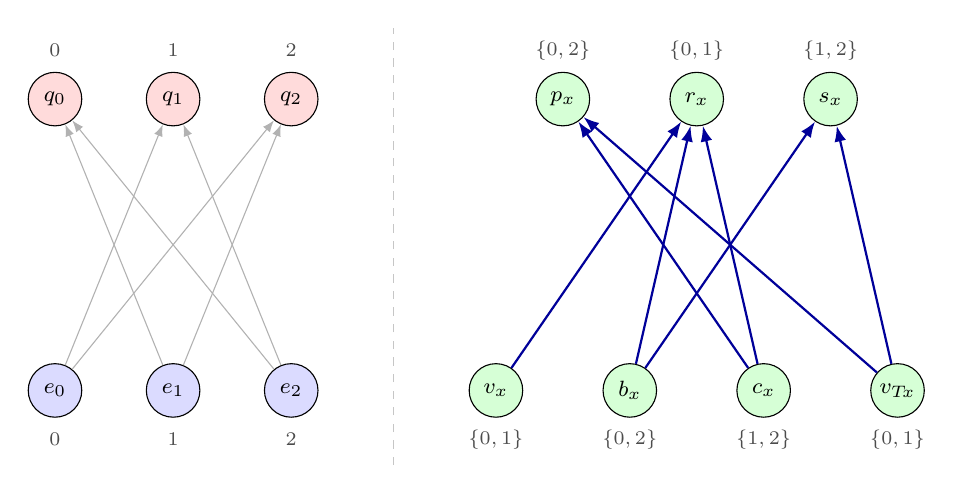
\begin{tikzpicture}[
				pt/.style={circle,draw,minimum size=6.8mm,inner sep=0.5pt,font=\footnotesize},
				anch/.style={pt,fill=blue!14},
				ref/.style={pt,fill=red!14},
				gad/.style={pt,fill=green!16},
				dom/.style={font=\scriptsize,inner sep=1pt,text=black!70},
				forced/.style={-{Latex[length=2mm]},blue!60!black,thick},
				aux/.style={-{Latex[length=1.5mm]},gray!60}
				]
				\node[ref] (q0) at (0,3.7) {$q_0$};
				\node[ref] (q1) at (1.5,3.7) {$q_1$};
				\node[ref] (q2) at (3,3.7) {$q_2$};
				\node[anch] (e0) at (0,0) {$e_0$};
				\node[anch] (e1) at (1.5,0) {$e_1$};
				\node[anch] (e2) at (3,0) {$e_2$};
				\draw[aux] (e0)--(q1); \draw[aux] (e0)--(q2);
				\draw[aux] (e1)--(q0); \draw[aux] (e1)--(q2);
				\draw[aux] (e2)--(q0); \draw[aux] (e2)--(q1);
				\node[dom] at (0,-0.62) {$0$};
				\node[dom] at (1.5,-0.62) {$1$};
				\node[dom] at (3,-0.62) {$2$};
				\node[dom] at (0,4.32) {$0$};
				\node[dom] at (1.5,4.32) {$1$};
				\node[dom] at (3,4.32) {$2$};
				
				\node[gad] (vx)  at (5.6,0) {$v_x$};
				\node[gad] (bx)  at (7.3,0) {$b_x$};
				\node[gad] (cx)  at (9.0,0) {$c_x$};
				\node[gad] (vTx) at (10.7,0) {$v_{T\!x}$};
				\node[gad] (px) at (6.45,3.7) {$p_x$};
				\node[gad] (rx) at (8.15,3.7) {$r_x$};
				\node[gad] (sx) at (9.85,3.7) {$s_x$};
				\node[dom] at (5.6,-0.62)  {$\{0,1\}$};
				\node[dom] at (7.3,-0.62)  {$\{0,2\}$};
				\node[dom] at (9.0,-0.62)  {$\{1,2\}$};
				\node[dom] at (10.7,-0.62) {$\{0,1\}$};
				\node[dom] at (6.45,4.32) {$\{0,2\}$};
				\node[dom] at (8.15,4.32) {$\{0,1\}$};
				\node[dom] at (9.85,4.32) {$\{1,2\}$};
				
				\draw[forced] (vx)--(rx);
				\draw[forced] (bx)--(rx);
				\draw[forced] (cx)--(rx);
				\draw[forced] (cx)--(px);
				\draw[forced] (vTx)--(px);
				\draw[forced] (vTx)--(sx);
				\draw[forced] (bx)--(sx);
				
				\draw[gray!45,dashed] (4.3,-0.95) -- (4.3,4.6);
			\end{tikzpicture}
			\caption{Left: the anchors and references. Every anchored proper $3$-colouring
				$d$ has $d(e_i)=i$ by hypothesis and hence $d(q_i)=i$, since $q_i$ lies above
				the two anchors of colour $\neq i$. Right: the gadget over $x\in\T$. Only the
				relations (IV) are drawn; the relations (II) and (III), omitted for
				legibility, pin the two-element colour domains shown next to each node. The
				seven drawn edges force $d(v_{T(x)})=1-d(v_x)$.}
			\label{fig:gadget}
		\end{figure}
		
		\begin{figure}[ht]
			\centering
			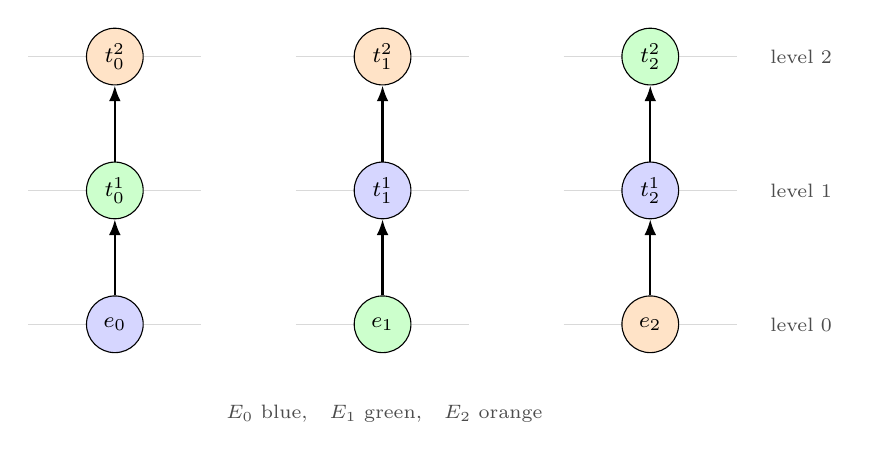
\begin{tikzpicture}[
				pt/.style={circle,draw,minimum size=7.2mm,inner sep=0.5pt,font=\footnotesize},
				b0/.style={pt,fill=blue!16},
				b1/.style={pt,fill=green!20},
				b2/.style={pt,fill=orange!22},
				up/.style={-{Latex[length=2mm]},thick},
				lab/.style={font=\scriptsize,text=black!70}
				]
				\foreach \c/\x in {0/0, 1/3.4, 2/6.8} {
					\draw[gray!30] (\x-1.1,0) -- (\x+1.1,0);
					\draw[gray!30] (\x-1.1,1.7) -- (\x+1.1,1.7);
					\draw[gray!30] (\x-1.1,3.4) -- (\x+1.1,3.4);
				}
				\node[b0] (e0) at (0,0) {$e_0$};
				\node[b1] (t01) at (0,1.7) {$t_0^{1}$};
				\node[b2] (t02) at (0,3.4) {$t_0^{2}$};
				\draw[up] (e0)--(t01); \draw[up] (t01)--(t02);
				
				\node[b1] (e1) at (3.4,0) {$e_1$};
				\node[b0] (t11) at (3.4,1.7) {$t_1^{1}$};
				\node[b2] (t12) at (3.4,3.4) {$t_1^{2}$};
				\draw[up] (e1)--(t11); \draw[up] (t11)--(t12);
				
				\node[b2] (e2) at (6.8,0) {$e_2$};
				\node[b0] (t21) at (6.8,1.7) {$t_2^{1}$};
				\node[b1] (t22) at (6.8,3.4) {$t_2^{2}$};
				\draw[up] (e2)--(t21); \draw[up] (t21)--(t22);
				
				\node[lab,anchor=west] at (8.2,3.4) {level $2$};
				\node[lab,anchor=west] at (8.2,1.7) {level $1$};
				\node[lab,anchor=west] at (8.2,0) {level $0$};
				\node[lab,anchor=north] at (3.4,-0.9)
				{\,$E_0$ blue,\quad $E_1$ green,\quad $E_2$ orange};
			\end{tikzpicture}
			\caption{The three saturating chains $e_j<t_j^{1}<t_j^{2}$, shaded by the
				block to which each point belongs. Every chain meets each of $E_0,E_1,E_2$
				exactly once, which is $\mathrm{(AS)}$; the three chains realise the three
				patterns $(E_0,E_1,E_2)$, $(E_1,E_0,E_2)$ and $(E_2,E_0,E_1)$, and this mixing
				of patterns is what prevents the argument of
				Remark~\ref{rem:order-compatible} from applying.}
			\label{fig:saturation}
		\end{figure}
		
		\emph{Forcing.} Let $d:X\to[3]$ be any proper colouring of the comparability
		graph of $P$ with $d(e_i)=i$ for $i<3$. By (I) the point $q_i$ lies above the
		two anchors whose colours are the elements of $[3]\setminus\{i\}$, so
		\[
		d(q_i)=i\qquad(i<3).
		\]
		Combining this with (II) and (III) confines $d$ on the gadget points to the
		domains
		\begin{gather*}
			d(v_x)\in\{0,1\},\qquad d(b_x)\in\{0,2\},\qquad d(c_x)\in\{1,2\},\\
			d(p_x)\in\{0,2\},\qquad d(r_x)\in\{0,1\},\qquad d(s_x)\in\{1,2\},
		\end{gather*}
		for every $x\in\T$. We claim that these domains together with (IV) force
		\begin{equation}
			d(v_{T(x)})=1-d(v_x)\qquad(x\in\T).
			\label{eq:forcing}
		\end{equation}
		
		Suppose $d(v_x)=0$. From $v_x<r_x$ and $d(r_x)\in\{0,1\}$ we get $d(r_x)=1$;
		from $c_x<r_x$ and $d(c_x)\in\{1,2\}$, $d(c_x)=2$; from $c_x<p_x$ and
		$d(p_x)\in\{0,2\}$, $d(p_x)=0$; and from $v_{T(x)}<p_x$ and
		$d(v_{T(x)})\in\{0,1\}$, $d(v_{T(x)})=1$.
		
		Suppose $d(v_x)=1$. From $v_x<r_x$, $d(r_x)=0$; from $b_x<r_x$ and
		$d(b_x)\in\{0,2\}$, $d(b_x)=2$; from $b_x<s_x$ and $d(s_x)\in\{1,2\}$,
		$d(s_x)=1$; and from $v_{T(x)}<s_x$, $d(v_{T(x)})=0$. This proves
		\eqref{eq:forcing}.
		
		\emph{(iii).} Suppose $d$ as above is Borel. Then $f:\T\to\{0,1\}$,
		$f(x)=d(v_x)$, is Borel, and \eqref{eq:forcing} says that $f$ is a proper
		$2$-colouring of $G_T$, contradicting Lemma~\ref{lem:rotation}. Since a Borel
		partition $X=A_0\sqcup A_1\sqcup A_2$ into antichains with $E_i\subseteq A_i$
		yields such a $d$, namely $d(x)=i$ for $x\in A_i$, no such partition exists.
		
		\emph{(i).} By Lemma~\ref{lem:rotation} choose a proper $2$-colouring
		$f:\T\to\{0,1\}$ of $G_T$, so $f(T(x))=1-f(x)$. Define $d$ on $X$ by
		$d(e_i)=d(q_i)=i$, by $d(t_j^{\,n})=\pi_j(n)$, and on the fibre over $x$
		according to the table
		\[
		\begin{array}{c|ccccc}
			d(v_x)=f(x) & b_x & c_x & p_x & r_x & s_x\\\hline
			0 & 0 & 2 & 0 & 1 & 2\\
			1 & 2 & 1 & 2 & 0 & 1
		\end{array}
		\]
		We check that $d$ is proper. The comparable pairs are those listed in
		(I)--(V) together with $e_j<t_j^{\,2}$. For (I), $d(e_j)=j\neq i=d(q_i)$. For
		(V) and $e_j<t_j^{\,2}$, the three points $e_j,t_j^{\,1},t_j^{\,2}$ receive the
		three distinct values $j,\pi_j(1),\pi_j(2)$. For (II), (III) and (IV) one reads
		off the table. If $f(x)=0$ the fibre colours are
		$(v_x,b_x,c_x,p_x,r_x,s_x)=(0,0,2,0,1,2)$ and $d(v_{T(x)})=1$, so the pairs
		of (II) are $0\!\neq\!2$, $0\!\neq\!1$, $2\!\neq\!0$; those of (III) are
		$1\!\neq\!0$, $2\!\neq\!1$, $0\!\neq\!2$; and those of (IV) are $0\!\neq\!1$,
		$1\!\neq\!0$, $1\!\neq\!2$, $0\!\neq\!1$, $0\!\neq\!2$, $2\!\neq\!0$,
		$2\!\neq\!1$. If $f(x)=1$ the fibre colours are $(1,2,1,2,0,1)$ and
		$d(v_{T(x)})=0$, and the same lists read $1\!\neq\!2$, $2\!\neq\!1$,
		$1\!\neq\!0$; $1\!\neq\!2$, $2\!\neq\!0$, $0\!\neq\!1$; and $1\!\neq\!0$,
		$0\!\neq\!2$, $0\!\neq\!1$, $2\!\neq\!0$, $2\!\neq\!1$, $1\!\neq\!2$,
		$1\!\neq\!0$. In both cases $d$ is proper, and $d(e_i)=i$ together with
		$d(t_j^{\,n})=\pi_j(n)$ gives $d^{-1}(\{i\})\supseteq E_i$. So
		$A_i=d^{-1}(\{i\})$ is an extension, and $\mathrm{(FE)}_3$ follows by
		restriction, or by Proposition~\ref{prop:compactness}.
		
		\emph{(ii).} Fix $j<3$. The chain $e_j<t_j^{\,1}<t_j^{\,2}$ has three
		elements and meets $E_j$ in $e_j$ and each $E_i$ with $i\neq j$ in the single
		point $t_j^{\,\pi_j^{-1}(i)}$. This one chain witnesses $\mathrm{(AS)}$ for
		$e_j$ and for both saturating points above $e_j$; as $j$ ranges over $[3]$ all
		nine points of $E_0\cup E_1\cup E_2$ are covered.
		
		\emph{Failure of $\mathrm{(AD)}$.} Take $t=1$, so $I_1=\{1,2\}$, and
		\[
		Z=E_1\cup E_2\cup\{q_0\}
		=\{e_1,t_0^{\,1},t_2^{\,2},e_2,t_0^{\,2},t_1^{\,2},q_0\},
		\]
		a seven-element set. Then $E_{I_1}\subseteq Z$ and $Z\cap E_0=\varnothing$,
		since $e_0,t_1^{\,1},t_2^{\,1}\notin Z$. Moreover $\hgt(P\restr Z)=2$: the
		only points of $Z$ lying strictly above something in $Z$ are $t_0^{\,2}$,
		$t_1^{\,2}$, $t_2^{\,2}$ and $q_0$, and nothing of $Z$ lies above any of
		these, while $t_0^{\,1}$ has nothing of $Z$ below it, its only lower bound
		being $e_0$. Thus the clique number of $G^{<}\restr Z$ equals $2=|I_1|$, so
		$\mathrm{(AD)}$ would provide antichains $P_1\supseteq E_1$ and
		$P_2\supseteq E_2$ partitioning $Z$. But $e_1<q_0$ and $e_2<q_0$ by (I), with
		$e_1\in P_1$ and $e_2\in P_2$, so $q_0$ can lie in neither, a contradiction.
	\end{proof}
	
	\begin{remark}
		\label{rem:AS-free}
		Theorem~\ref{thm:D} shows that $\mathrm{(FE)}_3$ cannot replace
		$\mathrm{(AD)}$ in Theorem~\ref{thm:many}, and that adding $\mathrm{(AS)}$
		does not help. The reason $\mathrm{(AS)}$ does not help is visible in the
		construction: for antichains it is not a hypothesis at all. If $P$ is any
		Borel order of height at most $h$ and $E_0,\dots,E_{h-1}$ is a prescription by
		Borel antichains consisting of $\le_P$-minimal points and satisfying
		$\mathrm{(FE)}_h$, then attaching to each $e\in\bigcup_iE_i$ a fresh chain
		$e<(e,1)<\dots<(e,h-1)$ and declaring $(e,n)$ to lie in the block
		$\pi_j(n)$, where $e\in E_j$, produces a Borel order of the same height with
		an enlarged prescription satisfying $\mathrm{(FE)}_h$ and $\mathrm{(AS)}$,
		from which the original problem is recovered by restriction. The attachment is
		harmless precisely because nothing lies below a minimal point, so no
		comparabilities between old and new points arise, and the height, being a
		supremum over chains each of which is confined to one fibre, does not
		increase.
	\end{remark}
	
	\begin{remark}
		\label{rem:order-compatible}
		Call $\mathrm{(AS)}$ \emph{order-compatible} if the witnessing chain can
		always be taken increasing in the index, $x_0<_P\dots<_Px_{h-1}$ with
		$x_i\in E_i$. Order-compatible saturation trivialises the problem, for every
		$h$ and with no recourse to compactness or invariant separation: let
		$c:X\to[h]$ be a Borel map with $x<_Py\Rightarrow c(x)<c(y)$, as furnished by
		the Borel Mirsky theorem; along a witnessing chain $c$ is strictly increasing
		and takes $h$ values in $[h]$, so $c(x_i)=i$, whence $c(e)=i$ for every
		$e\in E_i$, and $A_i=c^{-1}(\{i\})$ is the desired Borel partition. In the
		order of Theorem~\ref{thm:D} order-compatibility must therefore fail, and one
		sees directly why: it would require two points below $e_2$, which with
		$e_2<q_0$ would produce a chain of four. Thus among the two forms of
		saturation only the order-compatible one carries information, and the three
		patterns realised in Figure~\ref{fig:saturation} are exactly what obstructs
		it.
	\end{remark}
	
	\subsection{Three chains: an open problem}
	\label{subsec:open}
	
	The counterexample of \S\ref{subsec:counterexample} is a counterexample about
	antichains, and the construction that produced it is not available for chains.
	
	\begin{question}
		\label{q:chains}
		Let $P$ be a Borel partial order of width three on a standard Borel space $X$
		and let $E_0,E_1,E_2$ be a prescription by Borel chains satisfying
		$\mathrm{(FE)}_3$ and $\mathrm{(AS)}$. Must it extend to a Borel partition of
		$X$ into three chains?
	\end{question}
	
	By Corollary~\ref{cor:two-orders}(a) the answer is affirmative for two chains,
	where $\mathrm{(FE)}_2$ alone suffices; by Theorem~\ref{thm:many} it is
	affirmative for three if $\mathrm{(AD)}$ is assumed and $\mathrm{(PU)}$ is
	available. So Question~\ref{q:chains} asks precisely whether the gap exhibited by
	Theorem~\ref{thm:D} on the antichain side is present on the chain side as well.
	
	Two remarks on what a counterexample would have to look like. First,
	$\mathrm{(AS)}$ cannot be arranged for free. The construction of
	Remark~\ref{rem:AS-free} attaches a chain above a minimal prescribed point, and
	this is a local operation. In the chain case one would have to attach
	antichains, hence \emph{incomparabilities}, and incomparability is not
	transitive: new points incomparable to a prescribed point are also incomparable
	to each other unless one specifies otherwise, and the width, being a global
	constraint, is destroyed. We know of no local way to embed a Borel order of
	width $w$ into one of the same width in which every prescribed point lies on a
	$w$-antichain meeting each block once.
	
	Second, by Remark~\ref{rem:order-compatible} dualised, a counterexample must mix
	the patterns in which the witnessing antichains meet the blocks; if all of them
	met $E_0,\dots,E_{k-1}$ in one and the same order with respect to some Borel
	chain decomposition, the problem would again trivialise. The following minimal
	example shows that mixing is consistent with everything else, so that no cheap
	obstruction is available: let $P$ consist of two disjoint two-element chains
	$a_0<a_1$ and $b_0<b_1$ with all cross pairs incomparable, and let
	$E_0=\{a_0,b_1\}$ and $E_1=\{a_1,b_0\}$. Then $\wdt(P)=2$, both $E_i$ are
	chains, $\mathrm{(AS)}$ holds with the witnessing antichains $\{a_0,b_0\}$ and
	$\{a_1,b_1\}$ realising both patterns, $\mathrm{(FE)}_2$ holds, and the
	prescription extends, namely by $A_i=E_i$; but no chain decomposition
	constructed by ranking can produce it. For width two this is subsumed by
	Theorem~\ref{thm:two}. Whether the phenomenon can be combined with an ergodic
	obstruction at width three, as in \S\ref{subsec:counterexample}, we do not know.
	
	
	\begin{thebibliography}{99}
		
		\bibitem{AharoniKorman1992}
		R.~Aharoni and V.~Korman,
		\emph{Greene--Kleitman's theorem for infinite posets},
		Order \textbf{9} (1992), 245--253.
		
		\bibitem{Berge1961}
		C.~Berge,
		\emph{F\"arbung von Graphen, deren s\"amtliche bzw.\ deren ungerade Kreise
			starr sind},
		Wiss.\ Z.\ Martin-Luther-Univ.\ Halle-Wittenberg (1961), 114--115.
		
		\bibitem{Berge1982}
		C.~Berge,
		\emph{$k$-optimal partitions of a directed graph},
		European J. Combin. \textbf{3} (1982), 97--101.
		
		\bibitem{Burgess1979}
		J.~P.~Burgess,
		\emph{Effective enumeration of classes in a $\Sigma^1_1$ equivalence relation},
		Indiana Univ. Math. J. \textbf{28} (1979), no.~3, 353--364.
		
		\bibitem{Cameron1986}
		K.~Cameron,
		\emph{On $k$-optimum dipath partitions and partial $k$-colourings of acyclic
			digraphs},
		European J. Combin. \textbf{7} (1986), 115--118.
		
		\bibitem{CarroyMillerVidnyanszky2021}
		R.~Carroy, B.~D.~Miller and Z.~Vidny\'anszky,
		\emph{On the existence of small antichains for definable quasi-orders},
		J. Math. Log. \textbf{21} (2021), no.~2, 2150005.
		
		\bibitem{Dilworth1950}
		R.~P.~Dilworth,
		\emph{A decomposition theorem for partially ordered sets},
		Ann. of Math. \textbf{51} (1950), 161--166.
		
		\bibitem{Frank1980}
		A.~Frank,
		\emph{On chain and antichain families of a partially ordered set},
		J. Combin. Theory Ser. B \textbf{29} (1980), 176--184.
		
		\bibitem{Gao2009}
		S.~Gao,
		\emph{Invariant Descriptive Set Theory},
		Pure and Applied Mathematics \textbf{293}, CRC Press, Boca Raton, 2009.
		
		\bibitem{Greene1976}
		C.~Greene,
		\emph{Some partitions associated with a partially ordered set},
		J. Combin. Theory Ser. A \textbf{20} (1976), 69--79.
		
		\bibitem{GreeneKleitman1976}
		C.~Greene and D.~J.~Kleitman,
		\emph{The structure of Sperner $k$-families},
		J. Combin. Theory Ser. A \textbf{20} (1976), 41--68.
		
		\bibitem{HarringtonMarkerShelah1988}
		L.~Harrington, D.~Marker and S.~Shelah,
		\emph{Borel orderings},
		Trans. Amer. Math. Soc. \textbf{310} (1988), no.~1, 293--302.
		
		\bibitem{Kada1989}
		K.~Kada,
		\emph{Une version bor\'elienne du th\'eor\`eme de Dilworth},
		th\`ese, Universit\'e Paris~VI, 1989.
		
		\bibitem{Kechris1995}
		A.~S.~Kechris,
		\emph{Classical Descriptive Set Theory},
		Graduate Texts in Mathematics \textbf{156}, Springer, New York, 1995.
		
		\bibitem{KechrisSoleckiTodorcevic1999}
		A.~S.~Kechris, S.~Solecki and S.~Todorcevic,
		\emph{Borel chromatic numbers},
		Adv. Math. \textbf{141} (1999), no.~1, 1--44.
		
		\bibitem{Linial1981}
		N.~Linial,
		\emph{Extending the Greene--Kleitman theorem to directed graphs},
		J. Combin. Theory Ser. A \textbf{30} (1981), 331--334.
		
		\bibitem{Lovasz1972}
		L.~Lov\'asz,
		\emph{Normal hypergraphs and the perfect graph conjecture},
		Discrete Math. \textbf{2} (1972), 253--267.
		
		\bibitem{Miller2012}
		B.~D.~Miller,
		\emph{The graph-theoretic approach to descriptive set theory},
		Bull. Symbolic Logic \textbf{18} (2012), 554--575.
		
		\bibitem{Mirsky1971}
		L.~Mirsky,
		\emph{A dual of Dilworth's decomposition theorem},
		Amer. Math. Monthly \textbf{78} (1971), 876--877.
		
		\bibitem{Saks1979}
		M.~Saks,
		\emph{A short proof of the existence of $k$-saturated partitions of partially
			ordered sets},
		Adv. in Math. \textbf{33} (1979), 207--211.
		
	\end{thebibliography}
	
\end{document}
